%!TEX root = ../template.tex
%%%%%%%%%%%%%%%%%%%%%%%%%%%%%%%%%%%%%%%%%%%%%%%%%%%%%%%%%%%%%%%%%%%%
%% chapter4.tex
%% NOVA thesis document file
%%
%% Chapter with lots of dummy text
%%%%%%%%%%%%%%%%%%%%%%%%%%%%%%%%%%%%%%%%%%%%%%%%%%%%%%%%%%%%%%%%%%%%

\typeout{NT FILE chapter4.tex}%
\chapter{System Design}
\label{cha:system_design}
This chapter presents the overall design and conceptualization of the system developed. It begins in Section \ref{sec:requirements} with a description of the system requirements, followed by an overview of the system architecture in Section \ref{sec:architecture} and database structure in Section \ref{sec:database}.
Finally, it ends with a discussion of the implementation choices made during development, in Section \ref{sec:discussion_design}.

\section{Requirements}
\label{sec:requirements}

This section describes the requirements of this dissertation, categorized into the following areas: Interactive Map, \gls{3D} Model Interaction, and \gls{VR} environment.


\subsection*{Interactive Map}
A map of the Troia archaeological site under study was incorporated into the project to offer interactive functionalities.
\begin{itemize}
    \item \textbf{Map Navigation:} Users can navigate in the environment, and explore different locations.
    \item \textbf{Perspective Switching:} Toggle between top-down and profile views for better spatial understanding.
    \item \textbf{Layer Toggle:} Toggle visibility of layers, overlay a \textit{.tif} map illustration, such as excavation campaigns.
\end{itemize}

\subsection*{\gls{3D} Models \& Interaction}
A focus on the interaction with \gls{3D} models, which are integrated into a \gls{VR} environment.
\begin{itemize}
    \item \textbf{Artifact Interaction:} Allows users to virtually manipulate the glass artefact models.
    \item \textbf{Contextual Overlay:} Display descriptive data about the artefact, such as its origin, period, and historical usage.
    \item \textbf{Reconstructed Models:} Showcase how artefacts would look originally (having in consideration characteristics such as: colourless glass, archaeological drawings and symmetry). 
    \item \textbf{3D Models Integration:} The user can zoom the map to visualize the perspective of a specific \gls{3D} model.
    %select a position to visualize the perspective of their 3D model.
\end{itemize}

\subsection*{\gls{VR} Environment}
\gls{VR} functionalities to provide an intuitive \gls{UX}, enabling interaction with the \gls{VE} through the use of \glspl{HMD}.
\begin{itemize}
    \item \textbf{Immersive Experience:} \gls{VR} allows users to immerse in a virtual tomb visit, enabling interaction with glass relics.
    \item \textbf{Device Accessibility:} Primarily user-friendly and enabling haptic interaction, while supporting \gls{VR} glasses as an emerging display option.
    \item \textbf{Localization \& Wayfinding:} 
    \begin{itemize}
        \item \textbf{\gls{POI}:} Use colors, text, visual markers, or direction arrows to emphasize and guide users to historically significant locations.
    \end{itemize}
   % \item \textbf{Multilingual Support:} Provide language options to ensure accessibility for an international audience.
\end{itemize}

\section{System Architecture}
\label{sec:architecture}

The system is divided into three application layers.
The \textbf{Presentation Layer} manages the \gls{VR} environment and its interaction with users. The \textbf{Application Layer} includes the management of Unity Requests, with the support of the framework "UnityWebRequest"\footnote{\url{https://docs.unity3d.com/6000.2/Documentation/ScriptReference/Networking.UnityWebRequest.html}}, acting as an intermediate between the Unity client and the database. 
The communication flow between these layers is managed through a Node.js \gls{REST} \gls{API}, chosen for its flexibility and lightweight design. 
Finally, the \textbf{Data Access Layer} contains the database, which stores all information related to object data, excavation, and object interventions. 
The architecture of the system can be observed in Figure \ref{fig:architecture}.
\begin{figure}[h!]
    \centering
    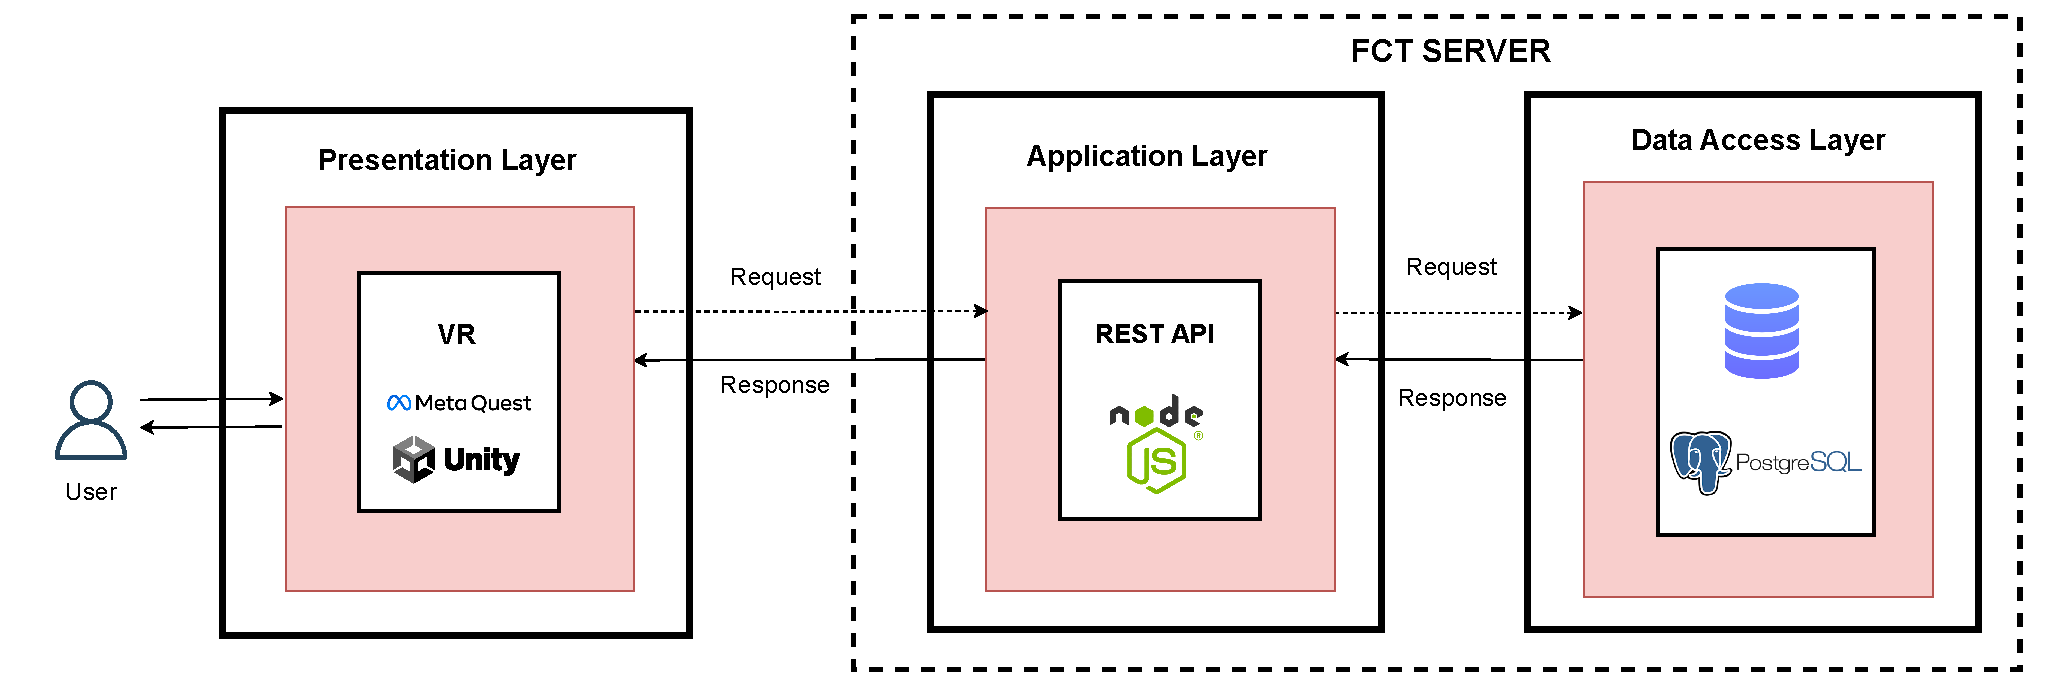
\includegraphics[width=1\linewidth]{Diagrama_Arquitetura}
    \caption{System Architecture Overview of the Developed System. \textcopyright\ Ana Maissa Antunes}
    \label{fig:architecture}
\end{figure}

During the development stage, the database was hosted locally on a PostgreSQL server managed via pgAdmin\footnote{\url{https://www.pgadmin.org/}}, an open source management tool for PostgreSQL. To access and present data in Unity, it was necessary to manually execute the "index.js" file, which contained the Node.js API endpoints.
Subsequently, before the user testing phase, the backend code, comprising both the \gls{API} endpoints and the PostgreSQL database, was deployed to the \gls{FCT} Server with a dedicated service.
This deployment ensured that the server hosting the \gls{API} endpoints remained continuously active, allowing Unity clients to retrieve data seamlessly without manual intervention.


\section{Database Structure}
\label{sec:database}

The database consists of 11 tables that ensure the significant data of excavation and objects are stored. %All artefacts data, excavation details, and objects intervention data were stored within this repository.
The database model was designed considering future extensibility. Initially, it was structured to store significant data from the necropolis, including the funerary enclosure and tomb under study. The structure was generalized to improve scalability, flexibility to possibly include data, such as other tombs, associated objects, and aggregate the maximum information. 
Throughout the thesis period, the database structure was continuously refined and restructured with new tables, relations, and data fields.

It was decided to not store the entire object images, as binary data in the database. Instead, only file paths to the images were saved. This allowed for efficient access and manipulation of images, while other object-related data, such as text and links, was fully stored in the database.

% The hierarchy of the tables is as follows: 
% \begin{itemize}
%     \item \textbf{necropolis} – the top-level table storing general information about the site.
%     \item \textbf{mausoleum} – representing the funerary enclosure and each record is linked to the necropolis id.
%     \item \textbf{tomb} – storing tomb data, and each record references the associated mausoleum via id foreign key.
%     \item \textbf{tomb\_belonger} – representing tomb belongers, and is linked to the tomb table via id foreign key.
%     \item \textbf{object} – storing information about individual objects, with 27 attributes describing each artifact.
%     \item \textbf{object\_intervention} – capturing interventions performed by \gls{VICARTE}, including the attributes \texttt{images\_path\_b\_interv} and \texttt{images\_path\_a\_interv} for images before and after intervention. This table references the \texttt{object} table through a foreign key.
%     \item \textbf{location} – storing coordinates for each object, linked via the object ID.
%     \item \textbf{excavation} – containing excavation details, with two child tables: \texttt{excavation\_protection} and \texttt{excavation\_area}, inheriting the excavation ID.
% \end{itemize}


The table \texttt{necropolis} is the top-level table and contains general information about the site.  
The funerary enclosure or mausoleum is represented by the table \texttt{mausoleum}, which stores information such as \emph{dimensions} and \emph{construction\_materials} and references the corresponding \emph{id} in \texttt{necropolis}. The tomb within the mausoleum is represented by the table \texttt{tomb} and has a foreign key \emph{id} referencing the associated mausoleum.  
While the table \texttt{tomb\_belonger} links tombs via its \emph{id}. The table \texttt{object} stores all information of each object, with 27 attributes describing each artifact. 
Moreover, table \texttt{object\_intervention} stores data about interventions performed by \gls{VICARTE}, including \emph{images\_path\_b\_interv} and \emph{images\_path\_a\_interv}, representing images of the object before and after the intervention. This table references the \emph{id} in the table \texttt{object}. Each object also has an associated table \texttt{location}, encompassing the coordinates of each object.  
Finally, the table \texttt{excavation} contains excavation information, with two child tables: \texttt{excavation\_protection} and \texttt{excavation\_area}, inheriting the \emph{id} of \texttt{excavation}.  

In Unity, only the following attributes are retrieved: from \texttt{object}, \emph{id}, \emph{name}, \emph{material}, \emph{provenance}, and \emph{dimensions}; from \texttt{object\_intervention}, \emph{images\_path\_b\_interv} and \emph{images\_path\_a\_interv}.

The detailed structure, including relationships and attributes, is illustrated in Figure \ref{fig:database}.

\begin{figure}[h!]
    \centering
    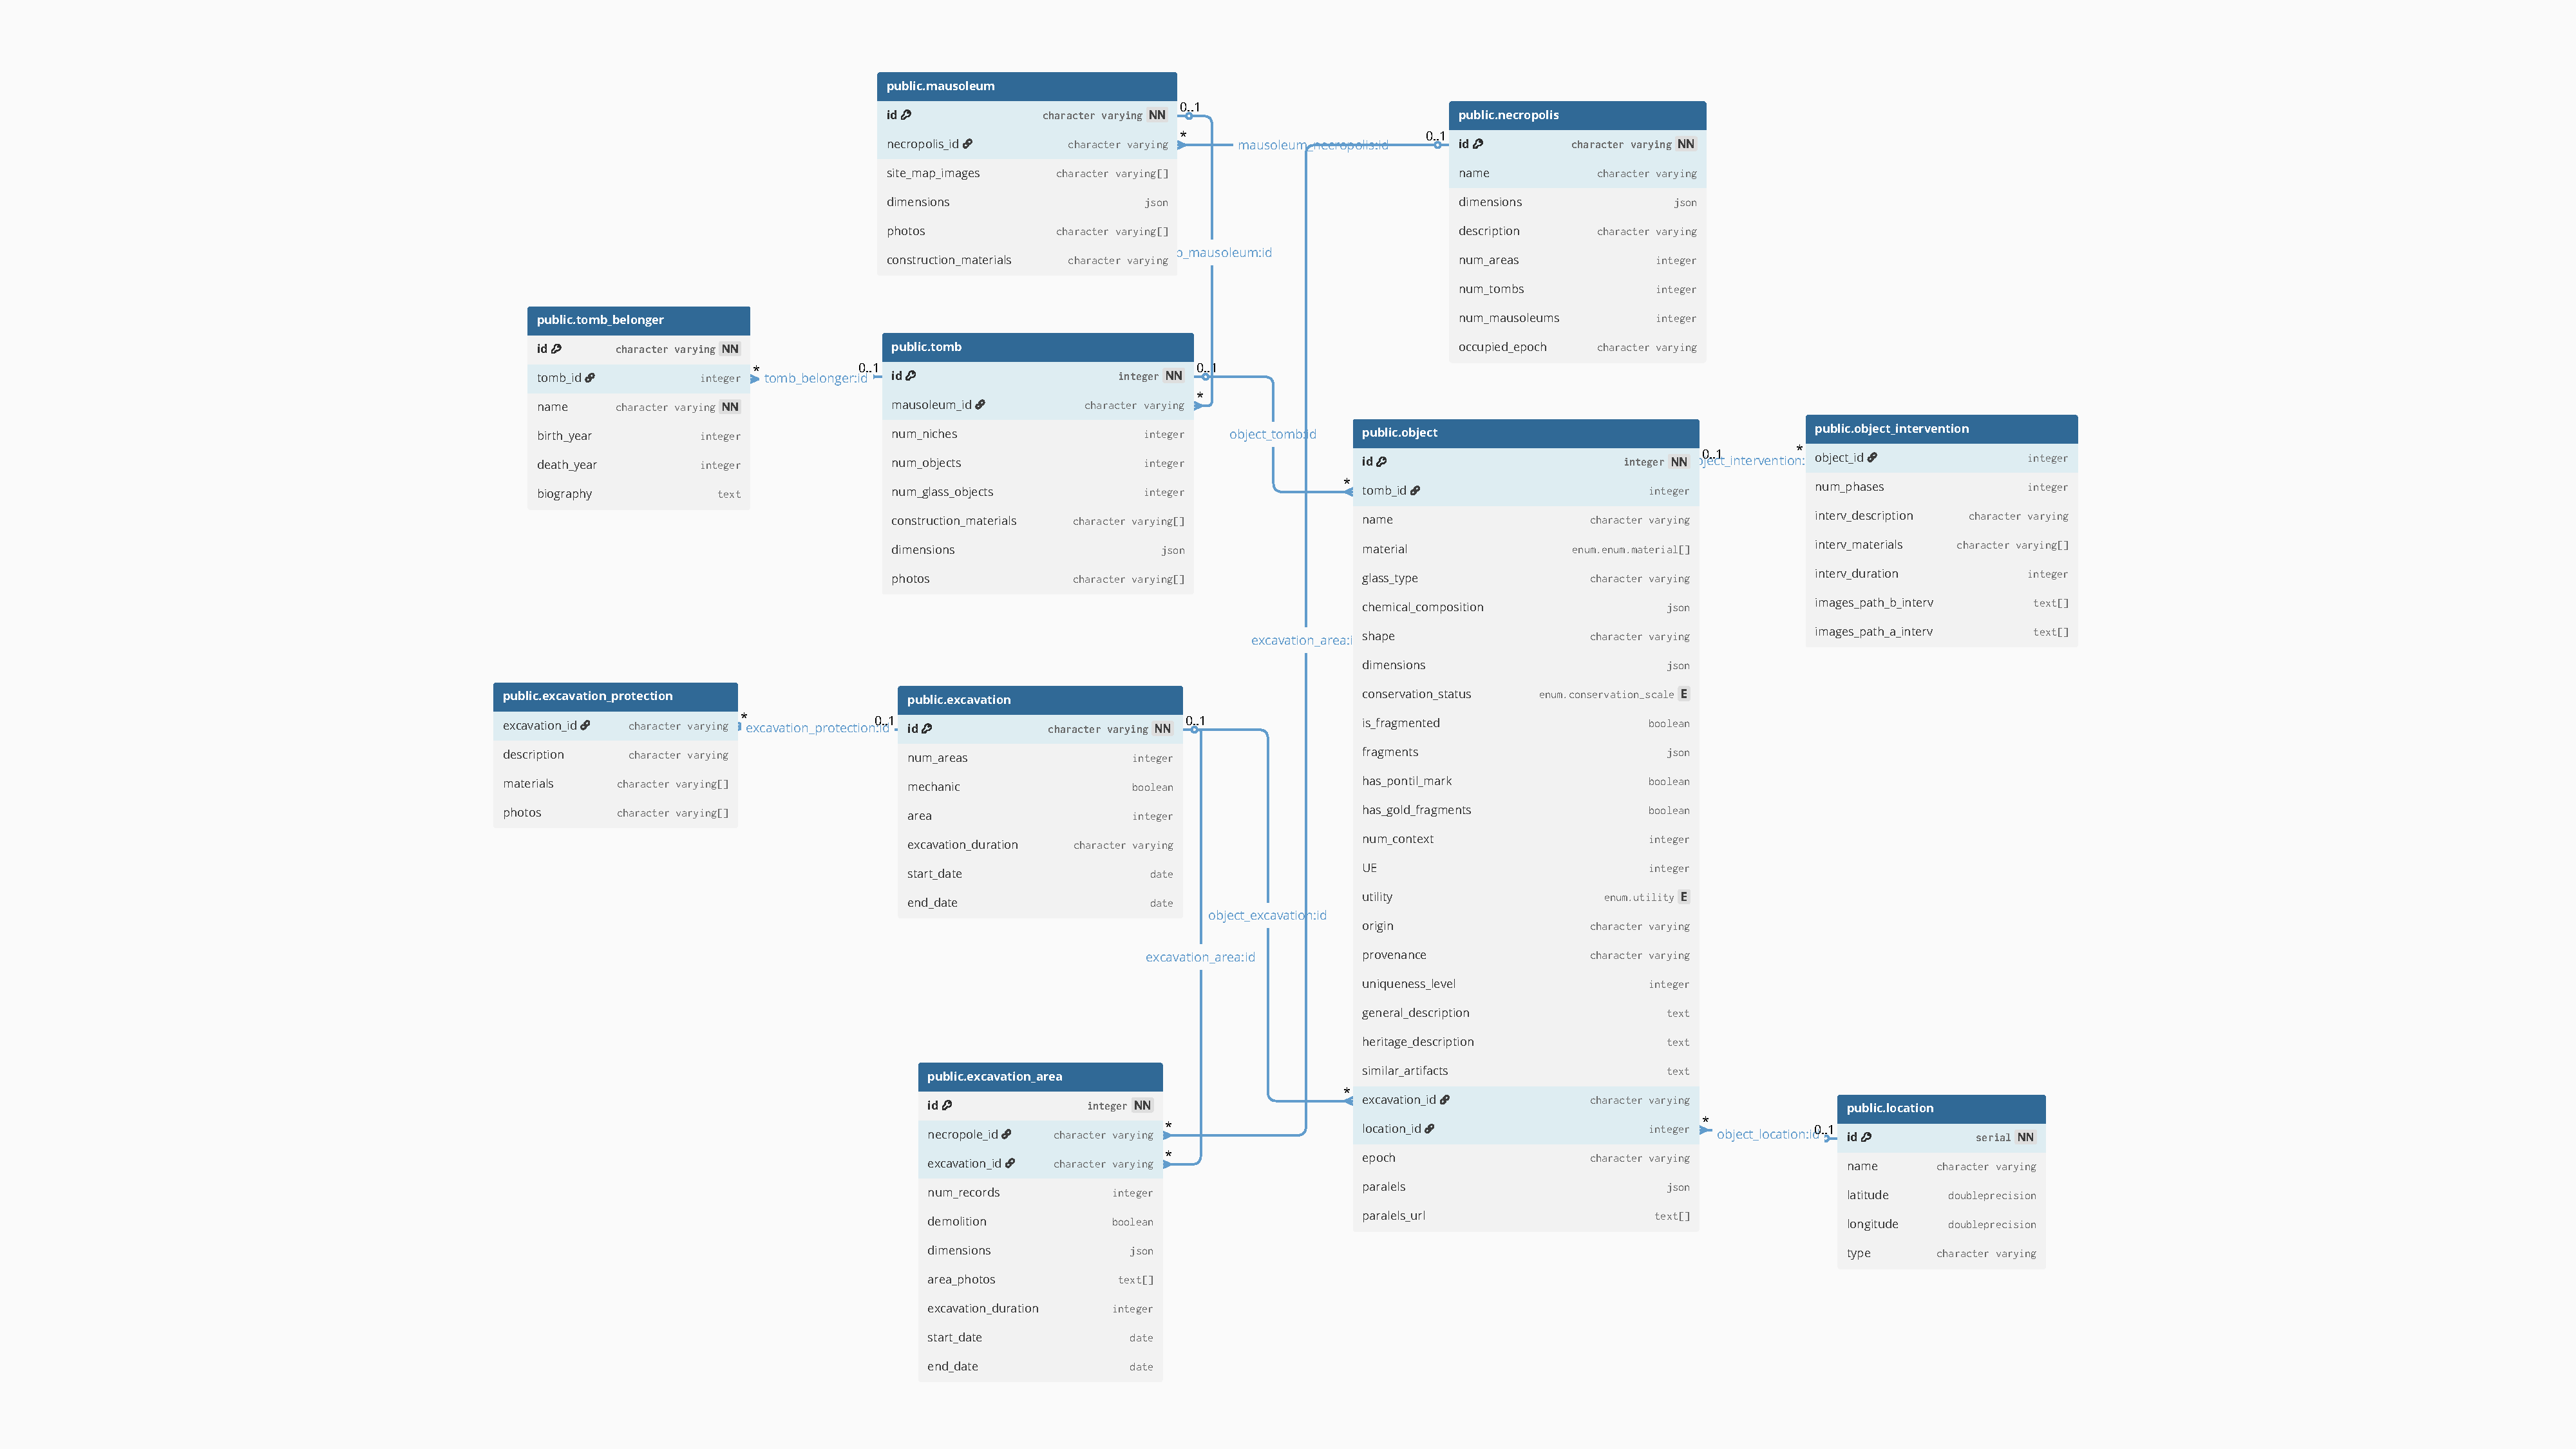
\includegraphics[width=1\linewidth, trim=13cm 0cm 13cm 0cm, clip]{thesis_db_}
    \caption{Relational Database Model.} 
    \label{fig:database}
\end{figure}


For generating the data model, SQL was used to create a database dump.
Using "dbdiagram.io", this dump was translated into a visual diagram showing tables and their relations. This tool streamlined the creation of the Entity-Relationship diagram through code.

\section{Discussion} %resumo do capitulo + opcoes tomadas
\label{sec:discussion_design}


Given the diverse requirements of this project, the primary focus was on developing an immersive \gls{VE}, prioritizing \gls{3D} models and \gls{VR} functionalities for exploring glass artifacts within the tomb. Although interactive map features were included, they were implemented with a lower level of detail.
At the beginning of the dissertation, the development of the \gls{VR} environment and the database proceeded in parallel. Once the base database structure was implemented, the main focus was on the construction of the \gls{VE}. The initial idea was to implement the map using JavaScript and the Leaflet.js\footnote{\url{https://leafletjs.com/}} library. However, the dissertation's direction shifted towards integrating the map with the funerary enclosure and its elements directly in Unity, forming a unified \gls{VE}. This allowed users to walk across the map as if in reality, while simultaneously visualizing the \gls{3D} models accurately positioned in space.

The implementation began with the integration of the map into Unity. 
Then, the model of the funerary enclosure was positioned on the map.
Following, the functionalities were implemented, such as \gls{3D} model visualization and map navigation, as outlined in Section \ref{sec:requirements}. 
Users can also grab objects, and interact with panel menus that displayed data retrieved from the database. 
A database was created to store significant data, including artefact and excavation data, with updates during development when needed. For interaction inside the tomb, two glass objects were chosen as the primary focus.

To enable communication between Unity and the database, a backend was implemented. Unity sent requests to the backend, which then queried the database and returned the requested information. 
A \emph{dropdown menu} was created in the \gls{VE} to fulfill requirement "Contextual Overlay", allowing the user to select an artefact ID and access the corresponding textual and visual data. 
Two request types were defined: (i) retrieval of all available ID from the "object" table, and (ii) retrieval of associated textual and image data, combining information from the "object" and "object\_intervention" tables.
For the layer toggle requirement, a photograph of the actual site was integrated, providing a stronger sense of presence for the user. Perspective switching was supported through photographs provided by specialists of the funerary enclosure architecture materials. 

The artefact reconstruction requirement was simplified: instead of reconstructing fragmented models, an illustration of the original object texture was simulated through the \emph{Object Slider} functionality.
As a result, users could enter the tomb and experience an immersive interaction with two glass relics, fulfilling the requirements of the \gls{VR} environment. Additional points of interest were distributed across the map to enrich the user experience.

Each functionality was tested individually, which was useful for correcting errors. After implementation, system testing evaluated the usability of the functionalities implemented to accomplish these requirements.





%The dissertation report was developed during the whole process.


